%%Berichtvorlage für EDBV WS 2014/2015

\documentclass[paper=A4, deutsch]{scrartcl}
\usepackage[ngerman]{babel}
\usepackage[utf8]{inputenc}
\usepackage{algorithmic}
\usepackage{algorithm}
\usepackage{graphicx}
\usepackage{amsmath,amssymb}
\usepackage{subcaption}
\captionsetup{compatibility=false}
\usepackage{multirow}
\usepackage{color}
\usepackage[]{geometry}
\graphicspath{ {./images/} }
\begin{document}


%%------------------------------------------------------
%% Ab hier tragt ihr eure Daten und Ergebnisse ein:
%%------------------------------------------------------

\title{nine-mans-morris} %%Projekttitel hier eintragen

\subtitle{EDBV WS 2018/2019: AG\_C3} %%statt XX Arbeitsgruppenbezeichnung hier eintragen (zB.: A1)


%%Namen und Matrikelnummern der Gruppenmitglieder hier eintragen
\author{Tobias Batik (11701221)\\
Bougouma Fall (01427956)\\
Yannic Ellhotka (11776168)\\
Simon Wesp (XXXXXXX)
}



%%------------------------------------------------------

\maketitle


%%------------------------------------------------------
\section{Gewählte Problemstellung}
(1-1,5 Seiten)\\
entspricht dem (aktualisierten) Konzept
\subsection{Ziel}
Ziel des Projekts\\
Brettspiel Muehle einlesen und moglichen naechsten Zug vorhersagen.
\subsection{Eingabe}
Folge von Farbbildern des Spielbrettes. 

\subsection{Ausgabe}
TODO müssen wir neu schreiben !!!!
\subsection{Voraussetzungen und Bedingungen}
Bilder muessen annaehernd in Volgelperspektive aufgenommen werden (+-30 Grad). \\
Das Spielbrett muss die in der Grafik dargestellten relativen Maßeinheiten erfüllen (siehe Abbildung 1) . 
Der Hintergrund der Spielfelder muss ausreichend Kontrast zu den weißen sowie schwarzen Spielsteinen aufweisen. \\
Die verwendeten Spielsteine haben eine durchmesser von Breite des Spielfelder * 0.08\\
Steine muessen eindeutig auf den vorgesehen Punkten liegen.\\

\begin{figure}[ht]
	\centering
		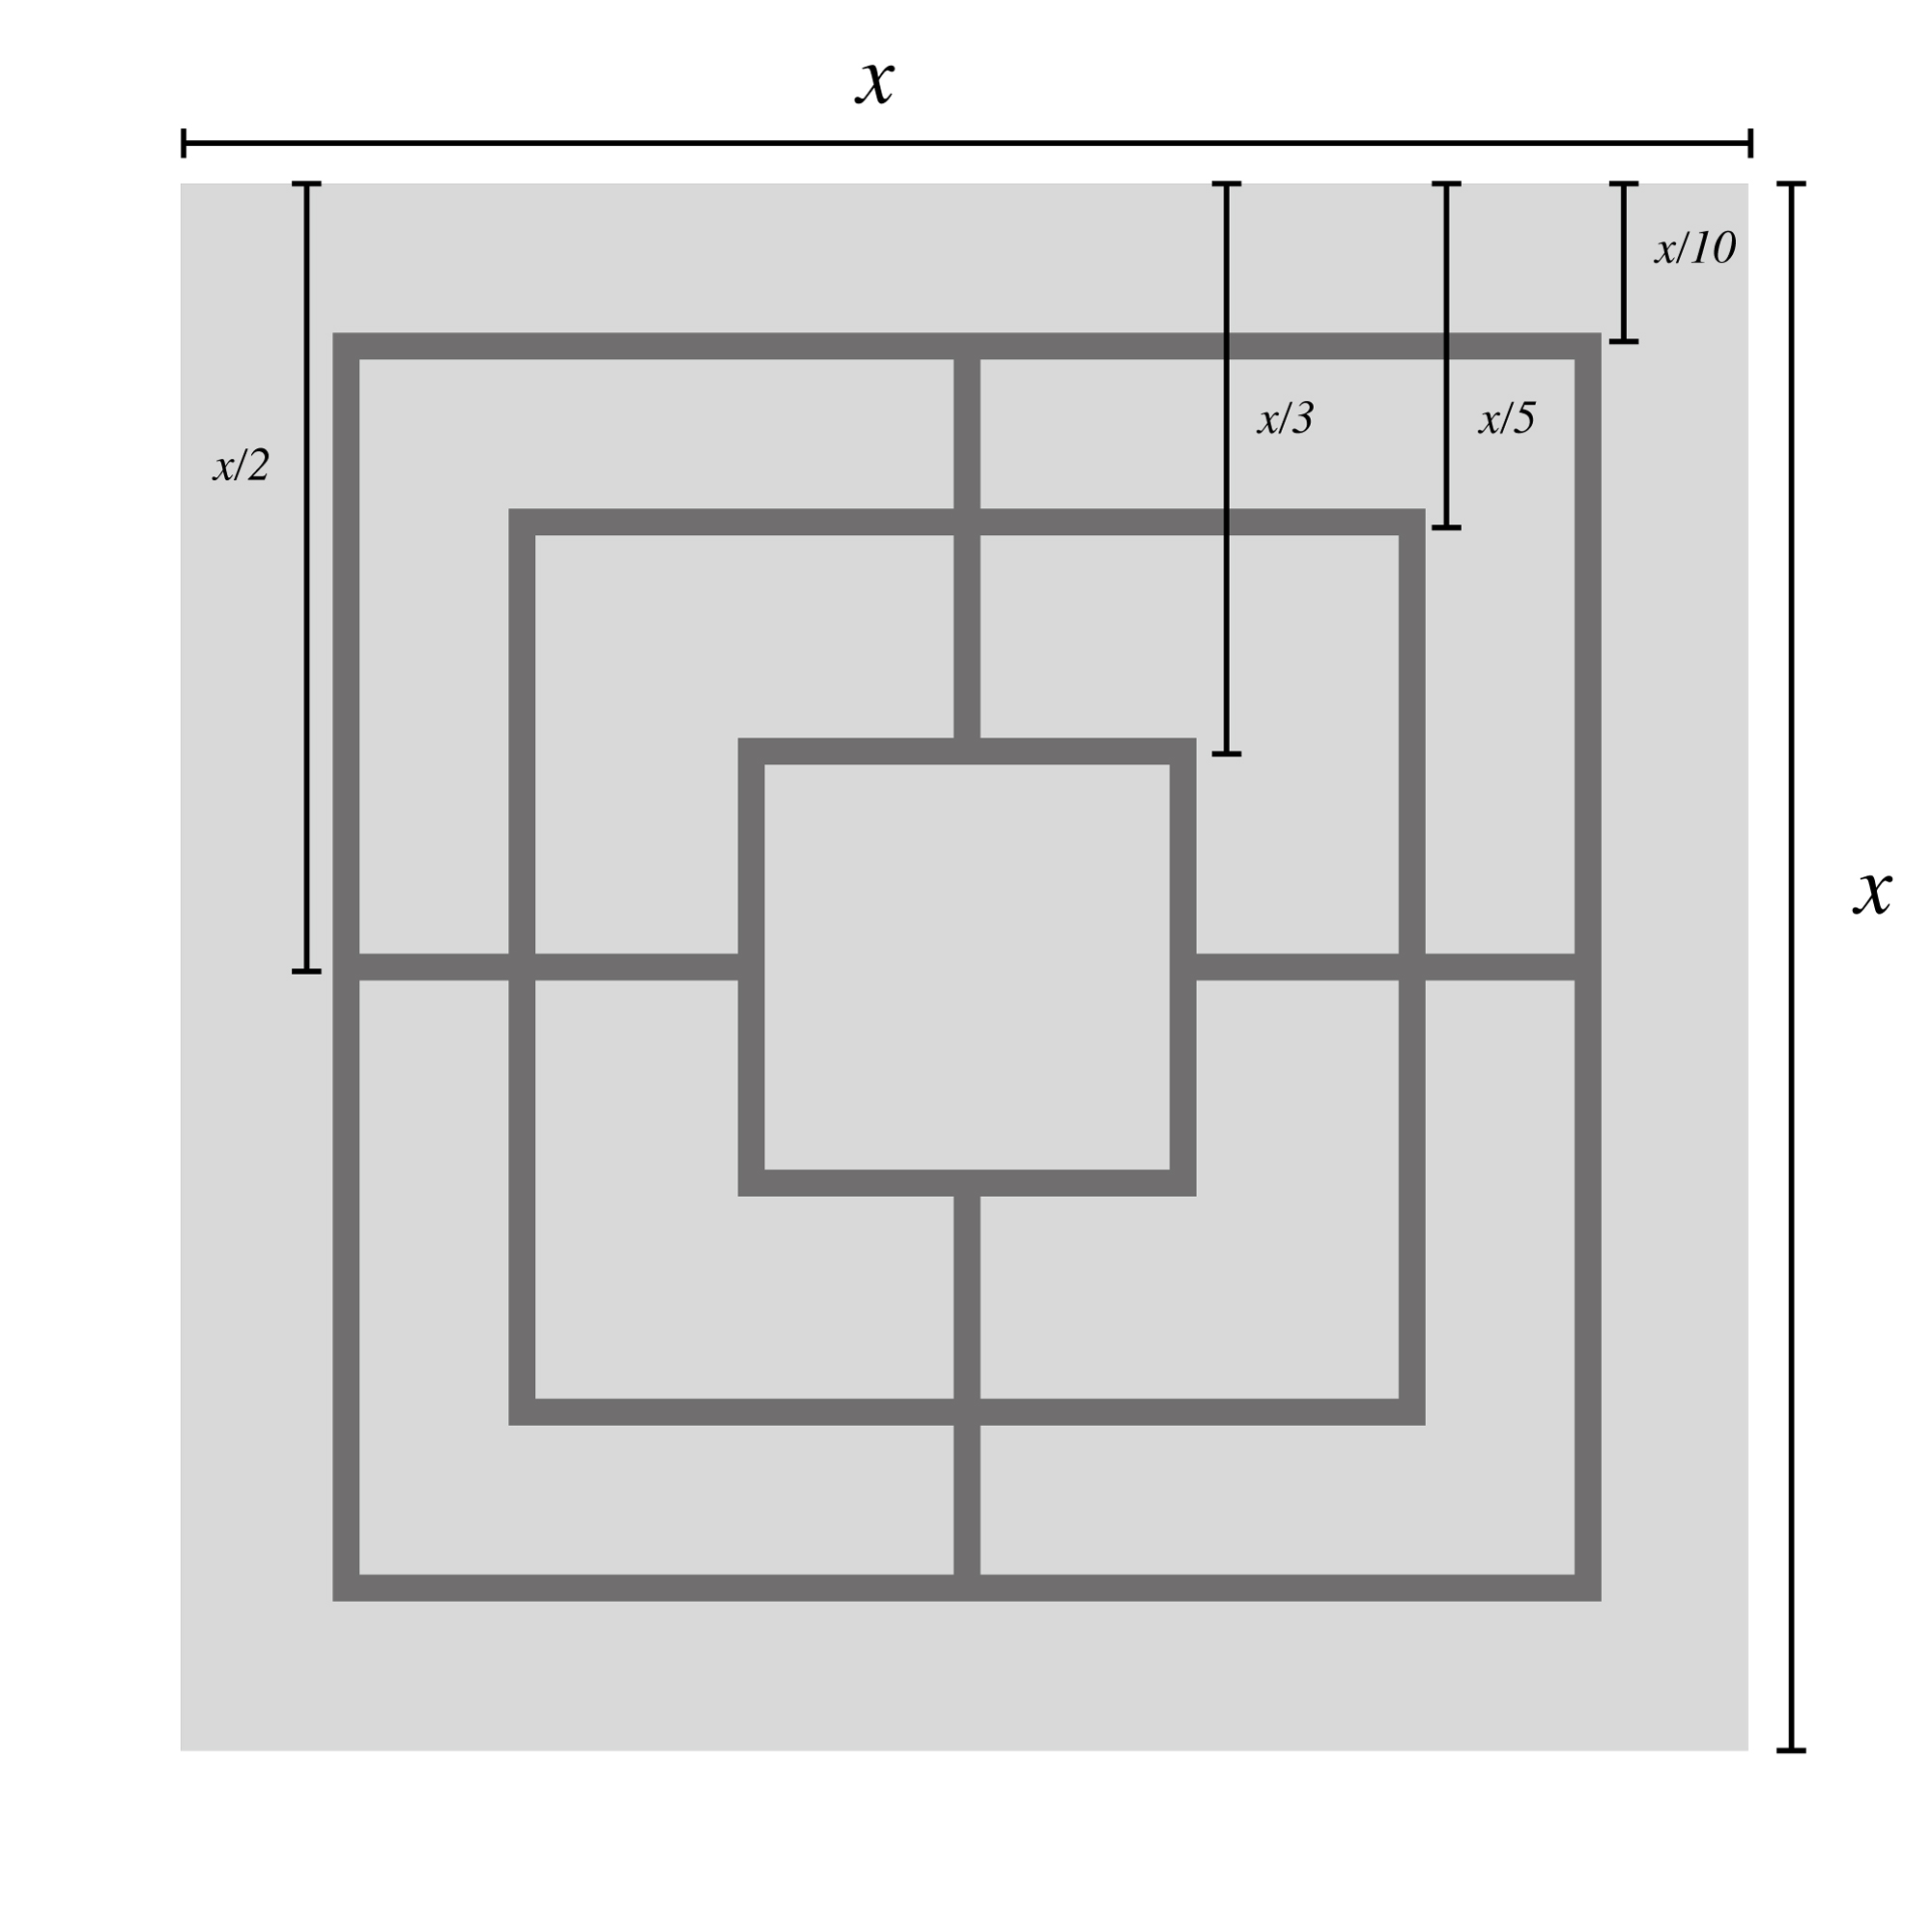
\includegraphics[width=8cm]{Spielbrett_relativeDimensionen_grafik.jpg}\\
	\caption[Relative Spielfelddimensionen]{Relative Spielfelddimensionen.}
	\label{fig:nettop}
\end{figure}



\subsection{Methodik}
1. Grauwert\\
\hspace*{1em} a. Input: RGB-Bild\\
\hspace*{1em} 	b. Output: Grauwertbild \\
2.  Threshold\\
\hspace*{1em} a. Input: Grauwertbild\\
\hspace*{1em} b. Output: Binärbild ???????? \\
3. Geometrische Transformation\\
\hspace*{1em} a. Input: Kantenbild und Koordinaten der Vierecke\\
\hspace*{1em} b. Output: transformiertes Kanten-Bild des Spielfeldes \\
4. Canny\\
\hspace*{1em} a. Input: Grauwertbild\\
\hspace*{1em} b. Output: Kantenbild \\
5. Hough-Transformation \\
\hspace*{1em} a. Input: transformiertes Kanten-Bild des Spielfeldes\\
\hspace*{1em} b. Output: Mittelpunkte der Spielsteine \\
6. Muss ich mir noch überlegen wie das heißt  \\
\hspace*{1em} a. Input: Mittelpunkte der Spielsteine und entzerrtes Graustufenbild\\
\hspace*{1em} b. Output: 3x3x3 Array das den aktuellen Spielstand repräsentiert \\
7. Algorithmus Zug berechnen Stimmt nicht mehr\\
\hspace*{1em} a. Input: Array des aktuellen Spielstands \\
\hspace*{1em} b. Output: Vorgeschlagener naaechster Zug

\subsection{Evaluierungsfragen}
1. Wird das Spielfeld richtig eingelesen?\\
2. Wird ein gueltiger Spielzug vorhergesagt?\\
\subsection{Zeitplan}
Der Zeitplan soll neben Euren anfänglichen, geplanten Zeiten/Arbeitsaufwände die tatsächlichen Zeiten/Arbeitsaufwände beinhalten. 
\begin{table}[h!]
	\centering
	\begin{tabular}{|c|c|c|c|c|}
		\hline
		Meilenstein & \multicolumn{2}{c|}{abgeschlossen am} & \multicolumn{2}{c|}{Arbeitsaufwand in h}\\
		\cline{2-5}
		 & geplant & tatsächlich & geplant & tatsächlich\\
		\hline
		...&... &... &... &...\\
		\hline
	\end{tabular}
\end{table}
%%------------------------------------------------------

%%------------------------------------------------------
\section{Arbeitsteilung}
(0,5 Seiten)\\
Wer hat welche Aufgaben übernommen (MATLAB-Funktionen, Abschnitt im Bericht, Evaluierung, Datenerfassung, etc.)? Die Aufteilung sollte fair sein, aber den tatsächlichen Aufwänden der einzelnen Teilnehmer entsprechen. Jeder übernimmt die Verantwortung (z.B. Korrektheit, keine Plagiate, wissen warum die Methode gewählt wurde) über seine ausgewiesenen Tätigkeiten.

\begin{center}
  \begin{tabular}{ |l | c | }
    \hline
  Name & Tätigkeiten\\
    \hline
		Tobias Batik & Matlab-Funktionen: hough, teilweise findStein; Bericht Abschnitt: 3.5, 4.5\\
		\hline
		Vorname2 Nachname2 & Matlab-Funktion C, Bericht Abschnitt D...\\
		\hline
		$\vdots$ & $\vdots$\\
  \end{tabular}
\end{center}

%%------------------------------------------------------

%%------------------------------------------------------
\section{Methodik}
(2-3 Seiten)\\
Hier wird die verwendete Methodik in der Theorie vorgestellt:\\
Welche Methodik wurde verwendet? Warum eignet sich diese Methodik für die gewählte Problemstellung? Habt ihr Methoden verändert (Einschränkungen, Abwandlungen, Parameter), wenn ja wie? etc.\\
Die erwähnten Methoden werden zum größten Teil auf Beschreibungen in Büchern oder wissenschaftlichen Artikeln beruhen. Daher ist hier auch der richtige Platz für Zitate. Die hier zitierten Publikationen sollten mittels Abkürzung bzw. Nummer referenziert sein und sich in der Referenzliste am Ende des Berichts über diese Bezeichnung finden lassen.\\
Ein Beispielsatz (inkl. entsprechender Literaturangabe am Ende des Berichts): Interest Points wurden mittels Scale Invariant Feature Transform \cite{lowe2004} detektiert.\\
Bei der Verwendung von Latex gestaltet sich das Zitieren besonders einfach - siehe Beispielssatz im Source der Latex-Vorlage.\\
\textbf{Wichtig in diesem Abschnitt ist, dass sich der Leser Eures Berichts mit den verwendeten Methodiken auskennt und weiß, weshalb ihr diese Methodiken verwendet habt und keine anderen. Es soll dem Leser helfen den nächsten Abschnitt des Berichts besser zu verstehen.}
\\
\\
\subsection{Hough Transformation für Kreise}
Zur erkennung der Kreisförmigen Spielsteine im entzerrtem Kantenbild kommt eine Hough-Transformation für Kreise zum Einsatz. \\
Die Kreis Hough Transformation ist ein übliches verfahren zum erkennen von Kreisen und deren Mittelpunkte. Das verfahren benötigt zur erkennung eines Kreises mit dem Radius \(c\) ein Set an Kantenpunkten die auf dem gesuchten Kreis liegen. 
	\footnote{\label{houghnote2} T.J Atherton, D.J. Kerbyson. "Size invariant circle detection." Image and Vision Computing. 
	Volume 17, Number 11, 1999, pp. 795-803.}\\
In einem Zweidimensionalen Raum kann ein Kreis mithilfe von \\
\begin{equation}
(x - a)^2 +(y - b)^2 = c^2 
\end{equation} 
beschrieben werden. \footnote{\label{houghnote1}R.O. Duda, P.E. Hart, Use of the Hough Transform to Detect Lines and Curves in Pictures, Communications of the ACM 15 (1972) 11– 15.
} Wobei der Punkt \((x,y) \)ein Kantenpunkt auf dem Kreis ist, \((a,b)\) der Kreismittelpunkt und \(c\) der Radius des Kreises.\\

Liegt eine Punkt \((x,y)\) auf einem Kreis im Eingabebild und ist der Radius \(c\) bekannt so k\"onnen alle Potenziellen Kreismittelpunkte \((a,b)\) mithilfe der oben erwähnten Formel ermittelt werden. Die Potenziellen Kreismittelpunkte werden in einem Akkumulator Array gespeichert. Die Maxima in diesem Array repräsentieren die gefunden Kreismittelpunkte.\footref{houghnote2} Siehe Abbildung \ref{fig:hough2d}.\\
\\
\begin{figure}[ht]
	\centering
		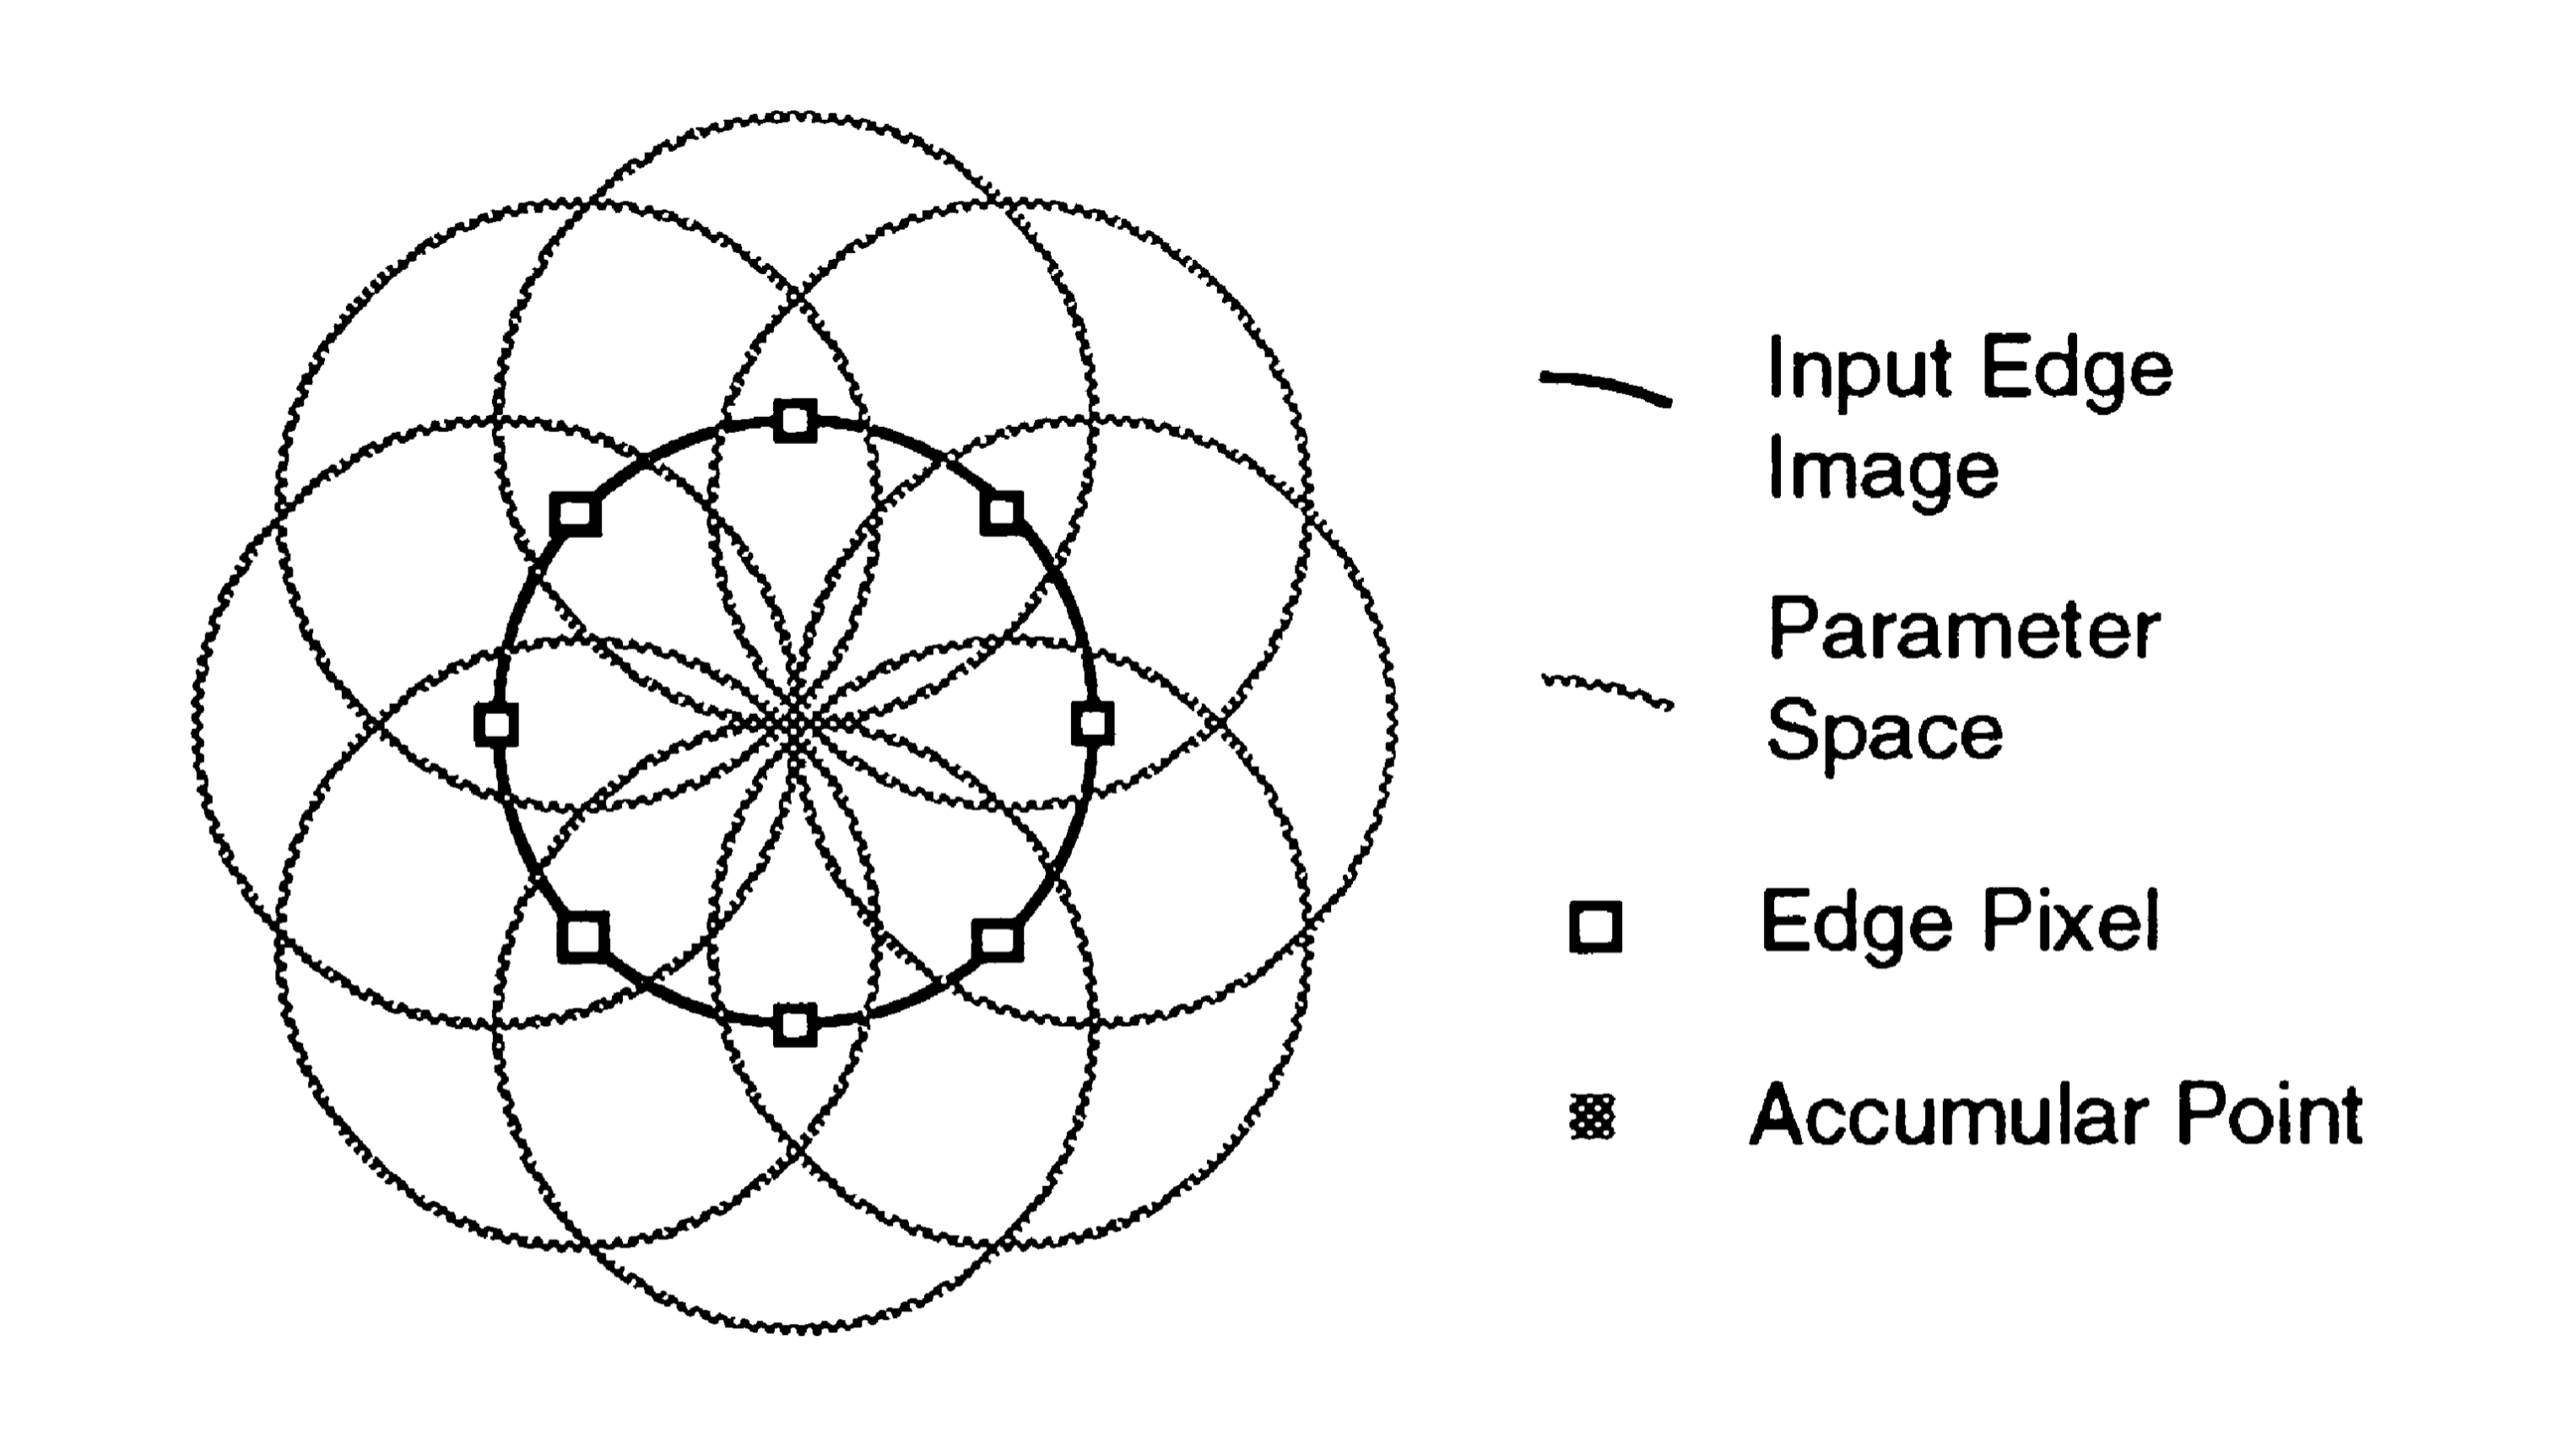
\includegraphics[width=6cm]{2dhough_darstellung.png}\\
	\caption[Funktion von Hough bei bekanntem Radius]{Funktion von Hough bei bekanntem Radius\footref{houghnote2}}
	\label{fig:hough2d}
\end{figure}

Wenn ein Punkt \((a,b,c)\) im Hough-Raum ein Maximum ist, so gibt es im Eingabebild einen Kreis mit dem Mittelpunkt \((a,b)\) und dem Radius  \(c\).\footref{houghnote1}
\\
\\
Visualisiert man die Potenziellen Kreismittelpunkte des Kantenpunktes als gerade Kreiszilinder im dreidimensionalens Hough-Raum, so repräsentiert der Schnittpunkt \((a,b,c)\) von Maximal vielen Zylindern den gefundenen Kreismittelpunkt \((a,b)\) mit dem Radius\( c\).






%%------------------------------------------------------

%%------------------------------------------------------
\section{Implementierung}
Die Implementierungspipeline sieht so aus, dass zuerst die Eckpunkte des Spielfelds mittels  einem Threshold erkannt werden. Die Eckpunkte werden dann verwendet, um das Spielfeld wieder zu einem perfekten Quadrat zu entzerren. Die Kanten des entzerrten Spielfelds werden mithilfe eines Canny Filters erkannt. Dabei sind nur die Kanten der Spielsteine wichtig da diese bei der Kreiserkennung verwendet werden. Der nächste Schritt ist, die Anwendung einer Hough Kreiserkennung auf das Canny Kantenbild, um die Position der Spielsteine zu ermitteln. Danach werden mit einer eigens endwickelten Methode die Spielsteine auf ein virtuelles, aus einem 3 x 3 x 3 Array bestehendes, Spielfeld gelegt. Der letzte Schritt ist der Vergleich von zwei Zügen (Bildern) und das Entscheiden ob dieser Zug gültig war. Dieser Schritt wird ebenfalls mit einem eigens endwickelten Algorithmus gelöst.

\subsection{Framework}
Das Framework ist so aufgebaut, dass alle 6 Methoden in einer Datei hintereinander, in einer for-Schleife, aufgerufen werden. Die Schleife läuft alle Bilder eins Spiels ab wobei es egal ist aus wie vielen Zügen ein Spiel besteht. Jede Methode liest jeweils ein Bild ein, verarbeitet dieses und speichert zum Schluss das verarbeitete Bild wieder ab.\\
In der Datei „main.m“ kann der User die Variable „game“ in Zeile 2 auf einen positiven Integer ändern, um auszuwählen welches Spiel analysiert werden soll. Ein weiterer Parameter, der vom User verändert werden kann, ist der Threshold, ebenfalls in der Datei „main.m“. Das Verändern der  Variable „threshold“ auf einen Wert zwischen 0 und 1 verändert die Stärke des Thresholds.\\
Um das Programm zu starten, muss der User lediglich die Datei „main.m“ in Matlab ausführen. Standardmäßig wird das erste Spiel im Datensatz komplett analysiert. Das Ergebnis wird in der Konsole ausgegeben. Dort kann der User sehen ob und wann unerlaubte Spielzüge auftreten.\\

\subsection{Threshold und Eckenerkennung}
Diese Methode liest RGB Bilder ein und gibt die 4 Eckpunkte des Spielfelds zurück. Außerdem wird das threshold Bild abgespeichert.\\
Als ersten Schritt wird das eingelesen Bild mittels der Matlab Methode „rgb2gray“ in ein Graustufenbild umgewandelt. Danach wird das Graustufenbild in ein Binärbild, mit der Methode „imbinarize“ und dem vom User definiertem threshold Wert, umgewandelt. Das Anwenden dieser 2 Methoden hintereinander hat bei unseren Tests bessere Ergebnisse erzielt als das alleinige Anwenden der Methode „imbinarize“. Um das Bild etwas zu säubern wird es anschließend mit einem  4 Pixel breitem kubischen Strukturelement erodiert. Das Ergebnis ist ein Binärbild in dem das Spielbrett weiß ist und der Hintergrund schwarz.\\
Mithilfe des Binärbildes können die Eckpunkte ermittelt werden. Es wird die Methode „find“ in Kombination mit „min“ und „max“ verwendet, um jeweils das erste und letzte weiße Pixel in einer Reihe und Spalte zu finden. Die roten Striche in dem nachfolgenden Bild sind jeweils auf Höhe des ersten weißen Pixels in +x, -x, +y und -y Richtung. Mithilfe von „min“ und „max“ können bei Koordinate der 4 Eckpunkte errechnet werden. Diese werden in einem Array abgespeichert und zurückgegeben.\\

\begin{figure}[ht]
	\centering
		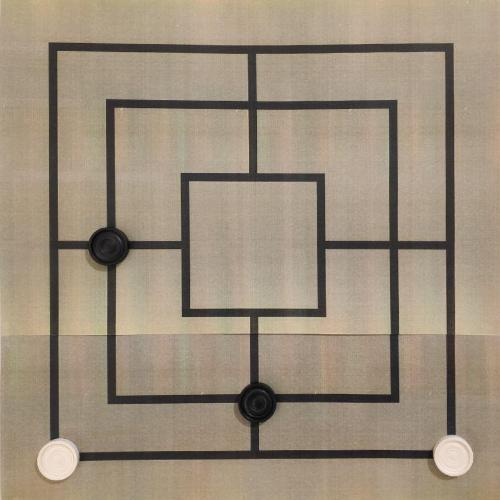
\includegraphics[width=8cm]{Spielbrett_Entzerrt.png}\\
	\caption[Spielfeld entzerrt]{Spielfeld entzerrt}
	\label{fig:nettop}
\end{figure}

\subsection{Geometrische Transformation}
Diese Methode liest das originale RGB Bild ein und bekommt die 4 Eckpunkte übergeben. Das Ergebnis ist ein 500 x 500 Pixel RGB Bild mit dem entzerrten Spielfeld wie man es an der nachfolgenden Bild sehen kann.\\

\begin{figure}[ht]
	\centering
		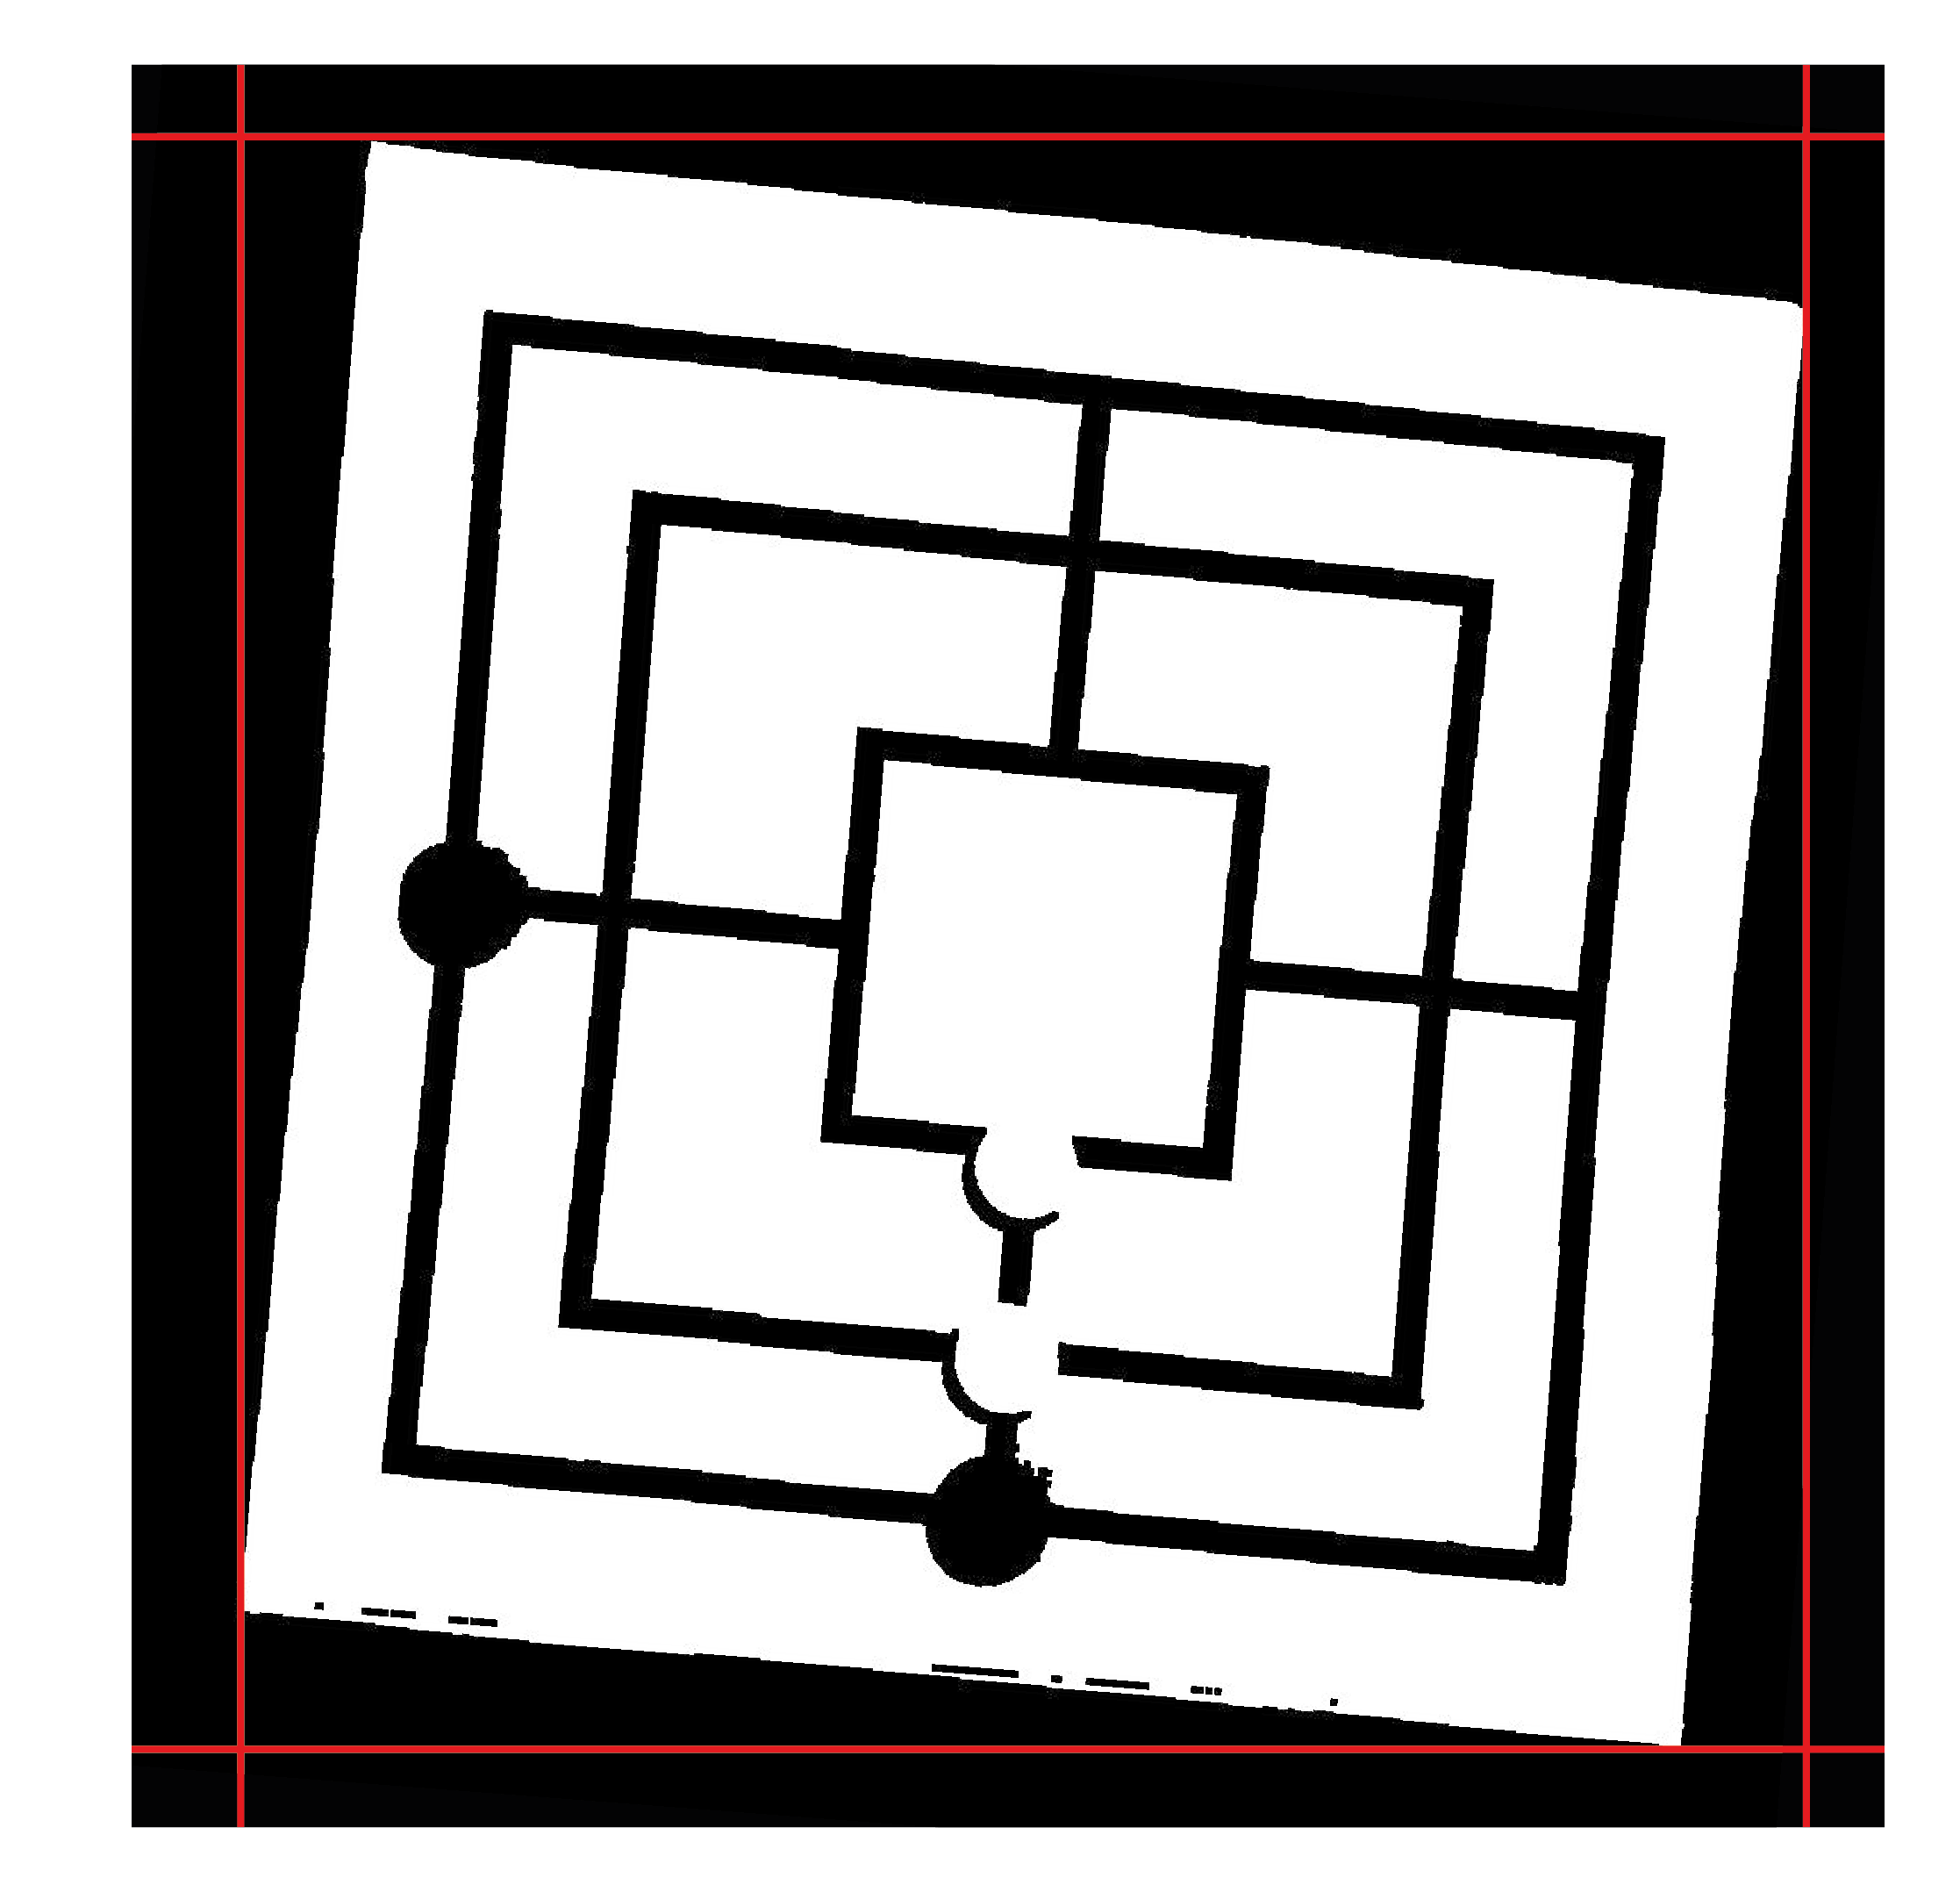
\includegraphics[width=8cm]{Ecken.png}\\
	\caption[Eckenerkennung]{Eckenerkennung}
	\label{fig:nettop}
\end{figure}

Geometrische Transformation ist der Überbegriff für viele verschiedene Anwendungen. In diesem Fall ist aber das entzerren eins perspektivischen Quadrates gemeint. Dazu werden die Eckpunkte des verzerrten Quadrates und die Größe des Quadrates in entzerrter Form benötigt. Nach dem Entzerren wird ein 500 x 500 Pixel Quadrat ausgeschnitten und abgespeichert\\
Zuerst muss die Transformationmatrix errechnet werden. Diese wird dann auf das verzerrte Bild angewendet, um dieses zu entzerren. Das Ergebnis ist ein Bild, in dem die 4 vorher definierten Punkte ein perfektes Quadrat bilden.\\
Die Koordinaten der jeweiligen Pixel ändern sich von Weltkoordinaten in Intrinsische Koordinaten nach der Transformation. Damit man das entzerrte Quadrat an den Eckpunkten ausschneiden kann, müssen die Eckpunkte zuerst in Intrinsische Koordinaten umgewandelt werden. Die Methode „imcrop“ mit den umgewandelten Koordinaten wird verwendet, um das Quadrat auszuschneiden. Das Ergebnis wird Abgespeichert.\\

\subsection{Canny Kantenerkennung}
Diese Methode liest ein entzerrte 500 x 500 Pixel RGB Bild ein und Speichert das dazugehörige Kantenbild ab.\\
Die Kantenerkennung nach Canny besteht aus einer Reihe von Schritten oftmals beginnend mit dem Anwenden eines Gauß’schen Weichzeichners auf das gesamte Bild. Weil das Spielfeld sehr klare Linien und Formen hat würde ein Weichzeichner das Ergebnis kaum verbessern, deshalb wird dieser Schritt in dieser Implementierung ausgelassen.\\
Der erste Schritt ist das Errechnen der Kantenkraft (wird für spätere Schritte benötigt), auch Magnitude genannt, indem man den Verlauf des Bildes mithilfe einer Sobel Matrix ausrechnet. Dieser Schritt muss jeweils in x- und y-Richtung durchgeführt werden.\\ 

\begin{figure}[ht]
	\centering
		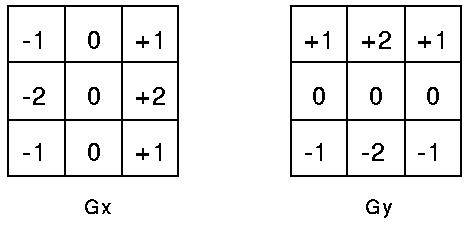
\includegraphics[width=8cm]{Sobel.png}\\
	\caption[Sobel Matrix]{Sobel Matrix}
	\label{fig:nettop}
\end{figure}

Die Länge der Hypotenuse der beiden Ankatheten Gx und Gy ist gleichzeitig auch die Magnitude.\\
Der nächste Schritt ist das Thresholding. Bei diesem Schritt werden Kantenpixel mit einem schwachen Magnitude Wert ausgefiltert. Das Ergebnis ist ein Kantenbild das nur starke Kanten enthält.\\
Der Letzte Schritt ist das Thinning, bei dem die Dicke der erkannten Kanten auf ein Pixel reduziert wird.\\

\subsection{Hough Kreiserkennung}
Die Funktion hough findet die Kreismittelpunkte von Kreisen mit einem Radius \(r\), \(radiusMin \leq r \leq radiusMax \)  und gibt diese als \(n * 2\) Matrix zurück. 
Um die Kreismittelpunkte zu finden liest die Funktion das Kantenbild des Aktuellen Spieles und Spielzug ein. \\
Die Funktion hough ruft für alle ganzzahliegen Radien (\(radiusMin \leq r \leq radiusMax\)) die Funktion hufffixedRadius auf und speichert alle gefundenen Mittelpunkte, unabhängig des Radiuses in einer einzigen Matrix (Radius wird nicht gespeichert da er für nächsten Schritte irrelevant ist).\\
\\


In der Funktion \(HoughFixedRadius\) wird über jedes Pixel des Kantenbildes iteriert. Falls das Pixel den Wert 1 hat, also ein Kantenpixel ist, werden m  viele potenzielle Kreismittelpunkte \((hy, hx)\)  abgeschlagen. Diese Punkte berechnen sich durch:  
\begin{equation}
hx = x + radius * cos(t)
\end{equation}
\begin{equation}
hy = y + radius *  sin(t)
\end{equation}
wobei \(t = (2\pi/m)*i\) ist. 
Im zweidimensionales Hough-Raum wird an der Stelle \((hy, hx)\) der Wert um eins erhöht. Siehe Abbildung \ref{fig:houghfixed}.\\

\begin{figure}[ht]
	\centering
		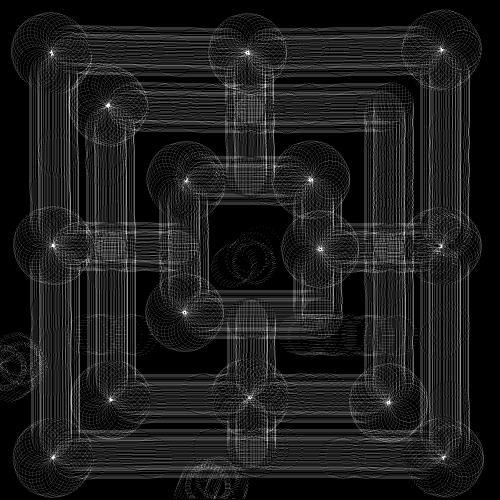
\includegraphics[width=8cm]{Huffexample3_16.jpg}\\
	\caption[Hough-Raum bei Radius = 20px]{Hough-Raum bei Radius = 20px}
	\label{fig:houghfixed}
\end{figure}

Anschließ end wird das Array auf Maxima untersucht. Da mehrere Kreise gefunden werden müssen, ist es nicht ausreichend das Array auf das Feld mit dem maximalen Wert zu bestimmen. Deshalb wird vom User der Wert \(minHoughValue\) gesetzt (zwischen 0 und 1). Ist der Wert \(minHoughValue = 0\) so wird jedes Feld im Hough-Raum als Kreismittelpunkt gedeutet deren Wert \(\geq 0\) ist. Ist \(minHoughValue = 1\) so werden nur jene Felder als Kreismittelpunkte aufgefasst deren Wert \(\geq amountCenterPoints\) ist.  Falls ein Feld im Hough-Raum als Kreismittelpunkt aufgefasst wird, wird die Position in einem Array gespeichert. \\
\\
Falls der Wert amountCenterPoints niedrieg gewählt wurde oder das eingelesene Kantenbild teilweise fehlerhaft ist. So kann es passieren das mehrer (leicht unterschiedliche) Kreismittelpunkte für den selben Kreis gefunden werden. Da nur die Mittelpunkte der Spielsteine relevant sind, wir davon ausgehen das alle Spielsteine annähernd gleich groß sind und dass nie zwei Spielsteine übereinander liegen dürfen, können alle gefundenen Kreismittelpunkte \((y_{j}, x_{j})\) deren Distanze \(d\) zum Kreismittelpunkt \((y_{i}, x_{i}) < Radius\) ist gelöscht werden. \\

Außerdem müssen wir beim Eingabebild voraussetzen, dass kein Runder gegenstand am Spielfeld liegt deren Radius \(r\)  \(radiusMin \leq r \leq radiusMax\) ist. 
Anschließend gibt die Funktion HoughFixedRadius alle gefundenen Kreismittelpunkte für den vorgegeben Radius zurück. \\

Da Handelsübliche Mühlesteine aus konzentrischen Kreisen aufgebaut sind kann es passieren, dass für einen Spielstein der selbe Mittelpunkt für unterschiedliche Radien gefunden wird.  Da wir wie oben erwähnt davon ausgehen dass nie zwei Steine übereinander liegen dürfen löschen wir wieder alle doppelt gefundenen Mittelpunkte. Mittelpunkte werden als Doppelt angesehn wenn die distanze zwischen den zwei Mittelpunkten kleiner als der kleinstmögliche Radius ist. \\

Anschließend wird ein .jpg Bild gespeichert wo die Kreismittelpunkte weiß Makiert sind, sowie ein .txt file mit den Kordinaten der gefundenen Kreismittelpunkte auf dem Eingabebild. Die Funktion Hough gibt die Kreismittelpunte als Matrix zurück. \\ 

\begin{figure}[ht]
	\centering
		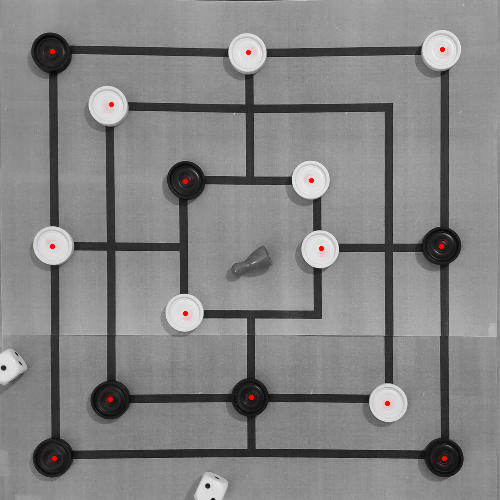
\includegraphics[width=8cm]{hough_performance.jpg}\\
	\caption[Gefundenen Kreismittelpunkte (rot) über dem entzerrten Graustuffenbild des Spielfeldes]{Gefundenen Kreismittelpunkte (rot) über dem entzerrten Graustuffenbild des Spielfeldes}
	\label{fig:hougresult}
\end{figure}


\subsection{findStein.m}

\subsection{Spiel Algorithms}


%%------------------------------------------------------

%%------------------------------------------------------
\section{Evaluierung}
(2-X Seiten)\\
Hier stellt ihr Euren Datensatz vor und beantwortet Evaluierungsfragen:\\
z.B. Fakten zum Datensatz: Anzahl der Bilder, Größe der Bilder, Quelle des Datensatzes (falls selbst aufgenommen: Aufnahmegerät, Einstellungen,... / falls nicht selbst erstellt: Datenbank vorstellen... $\to$ Referenzen!)\\
Diskussion der Evaluierungsfragen: Beantwortung der Fragen, Diskussion anhand von Beispielen, Diskussion von Grenzfällen: für welche Bilder funktioniert die Implementierung, für welche nicht? Worin unterscheiden sich diese Bilder? Warum funktionieren sie nicht? etc.\\
Evaluiert wird der ganze Datensatz, nicht nur einzelne Bilder. Einzelne Bilder können zum Aufzeigen von Fehlern/Problemen/besonders guten Ergebnissen... genutzt werden.\\
Zur Evaluierung gehört auch das Testen der einzelnen Methodiken (separat), mit Erwähnung eventueller Einschränkungen.
%%------------------------------------------------------

%%------------------------------------------------------
\section{Schlusswort}
(max. 1 Seite)\\
Hier fasst ihr Ergebnisse Eures Projekt zusammen:\\
Welche Schlussfolgerung lässt sich ziehen? Gibt es offene Probleme? Wie lässt sich Eure Lösung noch verbessern? etc.
%%------------------------------------------------------


%%------------------------------------------------------
\bibliographystyle{plain}
\bibliography{edbv_lit}
%%Bei verwendung von Latex schreibt ihr eure Referenzen in ein eigenes bib-File (siehe hier edbv_lit.bib). Jene Referenzen, die ihr im Bericht mittels \cite zitiert, werden automatisch in die Referenzliste übernommen. Weitere Information zum Einbinden von BibTex gibt es hier: http://www.bibtex.org/Using/de/
%%------------------------------------------------------
\textbf{Webseiten werden als Fußzeilen (an jener Stelle wo sie verwendet werden) eingebunden, nicht als Literature!}

\end{document}
\grid
\grid
